\section{Corpus-anchored supplemental transfer}\label{sec:transfer}
\subsection{Train-only corpus evidence and fixed follow-up protocol}
This extension follows instructor feedback and the original held-out analysis.
Before new scores, we fixed the corpus profile, transformations, cohorts, models,
contrasts and execution sources. It is a supplemental controlled follow-up on
\emph{already scored project test text}, not a new independent natural test or
blind preregistration. No retraining, checkpoint selection or hyperparameter
search uses these results. MultiLexNorm's test split remains unread; its lexical
normalization targets are not treated as punctuation-restoration gold.

The official Turkish training file contains 570 tweet/sentence records and
6,443 aligned slots; 354 split/merge slots are analyzed separately. Restricting
to one-to-one alphabetic Turkish/ASCII pairs permits target-preserving character
operations. A broader short-word-inclusive analysis finds 89 elongations among
4,512 eligible opportunities, 50 one-character internal omissions among 4,174,
and 43 partial folds among 621 words with multiple foldable occurrences. These
denominators include unchanged eligible pairs and differ by mechanism. They
must not be added or interpreted as percentages of all Turkish words.
Minimum word lengths are two for elongation, three for omission and two for
partial folding; partial folding additionally requires at least two foldable
occurrences and the casing compatibility described below.

The original surface-preserving folding map has a Turkish \texttt{I/\.I}
case-order incompatibility at four corpus opportunities. Excluding those words
and zero affected hits gives a separate \emph{operational} partial rate of
43/617; the earlier case-neutral 43/621 result is retained unchanged. Per-tweet
rate quartiles are all zero, so we use one empirical anchor per family rather
than invent natural mild/medium/heavy levels. Uniform whole-split target-word
sampling simplifies the corpus's observed tweet clustering.

For each family and seed, a new purpose-separated SHA-256 ranking selects exactly
$\lfloor N_{\mathrm{eligible}} h/o\rfloor$ clean word positions, where $h/o$ is
the relevant hit/opportunity ratio. On the primary test, elongation edits 3,355
of 170,103 eligible words, omission 1,826 of 152,483, and partial folding 1,803
of 25,881. The same selected words receive full folding as a seen-mechanism
control. Sensitivity filters these primary realizations without reranking.

Anonymous \emph{joint morphology templates}, rather than corpus vocabulary,
determine edits. Elongation retains ordered relative run positions and added
character counts: the 89 source events have median two extra characters,
maximum 25, and 12 multi-run cases. Feasibility-conditioned templates map to
distinct target character runs without clipping the tail. Omission deletes
exactly one internal character, preserving both endpoints; 47 uniquely aligned
events and three two-way ambiguous events contribute to a position distribution
with uniform ambiguity marginalization. Partial folding preserves available
count, changed count and relative sites jointly. Supported target counts use
their conditional profile; unsupported counts map a donor fraction to a nonempty
proper subset. This extrapolates 43/39/22 selected words at seeds586/587/588.
Conditioning, mapping and extrapolation are declared approximations to the
natural error process; exact rules and realized histograms are public.

Each of four fixed models receives a fresh clean anchor and four conditions at
each of three corruption seeds: $4(1+4\times3)=52$ forwards, or 104 cohort score
sets. The original T4/FP32/SDPA-math/batch16 policy, clean-length batch membership,
targets and first-subword alignment remain fixed. A separate runtime gate checks
all four actual checkpoints and 24 validation-only technical probes before
scoring. Saved-input checks and fresh tokenization retain every target, with
maximum length 154, no truncation and no condition-specific row filtering.
All saved predictions were independently rescored locally against original
targets; all 104 score sets match. Each fresh clean anchor also exactly matches
its original held-out counterpart in both cohorts.

\subsection{Complete results and bounded transfer}
\begin{table}[t]
\centering\footnotesize\setlength{\tabcolsep}{3pt}
\caption{Complete supplemental primary matrix, macro-F1 (\%). Noisy cells are
three-corruption-seed means $\pm$ sample SD. Without case uses the same selected
removal checkpoint; no model is retrained.}
\label{tab:transfer-primary}
\TransferPrimary
\end{table}

Augmented exceeds Clean on average under all three new mechanisms
(Table~\ref{tab:transfer-primary}): $+0.2491\pm0.0843$ pp for elongation,
$+0.2290\pm0.0635$ for omission and $+0.1882\pm0.0425$ for partial folding.
The matched full-folding control has $+0.1279\pm0.0446$ pp. These low-dose
differences are much smaller than the original combined-heavy gain; unlike
that stress test, these rates condition on mechanism-specific eligible words.
They are not a dose-matched severity comparison across studies or families.
All paired values, sensitivity results and unfavorable class differences are
retained (Table~\ref{tab:transfer-paired}, Appendix~\ref{app:transfer}).

\begin{table}[t]
\centering\footnotesize\setlength{\tabcolsep}{4pt}
\caption{Predefined supplemental paired differences (pp). P/S denote primary
and sensitivity. Each difference precedes aggregation within seed.}
\label{tab:transfer-paired}
\TransferPaired
\end{table}

Absolute noisy performance includes the existing $+0.1387$ pp clean-anchor
advantage. Own-anchor drops therefore provide a useful complementary view:
Clean/Augmented lose 0.2408/0.1304 pp under elongation, 0.1636/0.0732 under
omission and 0.0987/0.0492 under partial folding. This supports modest transfer
under these specific edits, without a significance or training-stability claim.
Retaining case loss gives small positive \emph{absolute} noisy-score means over
the removal arm (0.0816/0.1102/0.0579 pp). It does not uniformly reduce relative
degradation: Without case loses only 0.1215 pp on elongation and 0.0166 on partial
folding, less than Augmented. Thus this supplement does not establish that
case-loss training specifically protects against all three mechanisms.

\begin{figure}[t]
\centering
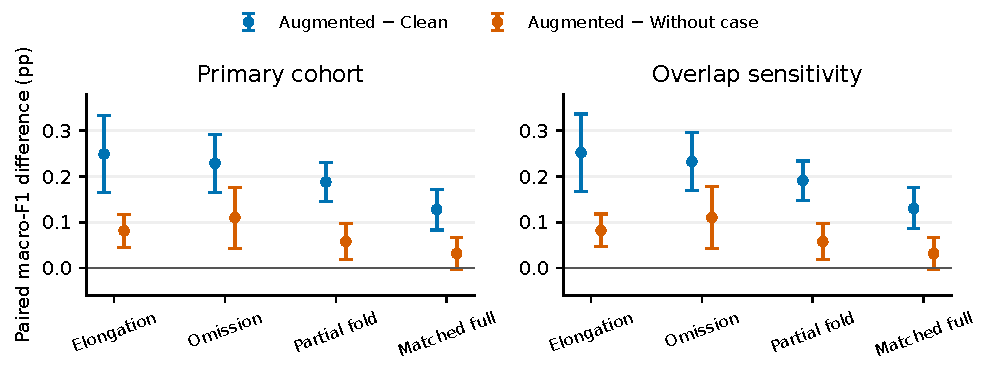
\includegraphics[width=\linewidth]{figures/transfer.pdf}
\caption{Supplemental paired contrasts. Error bars show corruption-seed SD,
not confidence intervals or training uncertainty. Matched full is a control;
character dose differs from partial folding.}
\label{fig:transfer}
\end{figure}

Class behavior remains uneven: for example, Augmented minus Clean elongation
F1 is negative for PERIOD (96.0856\% versus 96.1093\%) while positive for COMMA
and QUESTION. QUESTION has only 1,228 primary targets, compared with 15,465
PERIOD and 12,164 COMMA. Appendix~\ref{app:transfer} reports all four models'
class F1, supports, own-anchor drops and sensitivity matrix; full per-seed
P/R/F1 and four-class confusions accompany the public results.

The partial-minus-matched-full control has mixed model signs: Published
$-0.0522\pm0.0563$ pp, Clean $-0.0404\pm0.0361$, Augmented
$+0.0198\pm0.0424$, and Without case $-0.0062\pm0.0368$. Although both edit
the same 1,803 words per seed, partial folding changes 2,171/2,188/2,140
characters and full folding 4,762/4,772/4,777. Consequently these contrasts
cannot isolate whether a mechanism was explicitly seen during fine-tuning.
No global pooled robustness score or post-score recipe refinement is introduced.
